% title: thesis.tex
% author: see dukethesis.cls for list of contributors
% description: Duke PhD Thesis LaTeX Template

% NOTE: to compile this document, see the ./compile script

%% ---- preamble

% NOTE: template from: 
% https://gradschool.duke.edu/academics/theses-and-dissertations 
\documentclass[PhD]{dukethesis}

% imports
\usepackage{amsmath}
\usepackage{amssymb}
\usepackage{amsthm}
\usepackage{array}
\usepackage{xy}

% for double spacing
\usepackage[doublespacing]{setspace}

% for compact enumeration
% https://tex.stackexchange.com/a/43744/228201
\usepackage{paralist}

% for colors
\usepackage{xcolor}

% define any custom colors
%\definecolor{gray}{RGB}{240,240,240}

% for urls
\usepackage[hidelinks]{hyperref}
\hypersetup{colorlinks=true, linkcolor=black, citecolor=black, urlcolor=blue}

% for degree command
\usepackage{gensymb}

% for bibliography style (nature-like)
\usepackage[numbers, super, sort&compress]{natbib}
\setlength{\bibsep}{15pt} % approximate double spacing btw entries

% input graphics
\usepackage{graphicx}
\graphicspath{ {./graphics/} }

% for continued captions
% https://tex.stackexchange.com/questions/53315/how-to-put-large-figure-caption-on-separate-page-from-the-figure
\usepackage{ccaption}

% for dummy text
\usepackage{lipsum}  

% also from Duke Graduate School template:
%\input{macros.tex} 
% ^ I didn't use any of these macros. Try to keep things simple as possible.

% set space above and below fig captions
\setlength{\abovecaptionskip}{3pt plus 2pt minus 2pt} % default = 10
\setlength{\belowcaptionskip}{3pt plus 2pt minus 2pt} % default = 0

\author{First Last}
% NOTE: don't include title, e.g. Dr. or M.D.
\advisor{First Last} 
\member{First Last}
\member{First Last}
\member{First Last}

\department{Department}

% this should be title case
\title{
		\large{Doing Awesome Science and Finding Interesting Results}\\
		\small{High Impact Subtitle}
	}


%% ---- main

\begin{document}

\maketitle


%% ---- copyright

\Copyright


%% ---- abstract

%\makeabstract

\abstract

\lipsum[1]


%% ---- acknowledgments

\acknowledgements

I can only see so far because I stand on the shoulders of giants.

\lipsum[2-3]


%% ---- automatically generated loc, lof, lot

% these sections should be single spaced:
\begin{singlespace}
\tableofcontents

\listoffigures

\listoftables
\end{singlespace}

% abbrev are double spaced between entries
\section*{Abbreviations}

\begin{tabular}{ >{\bfseries}l l }
	APEX	 &  Ascorbate Peroxidase \\
	AMPA     &  Alpha-amino-3-hydroxy-5-Methyl-4-isoxazole Propionate \\
	AP-MS    &  Affinity Purification and Mass Spectrometry \\
	ASD      &  Autism Spectrum Disorder \\
	BioID	 &  Biotinylation Identification \\
	CNS	 &  Central Nervous System \\
	CRISPR   &  Clustered Regularly Interspaced Short Palindromic Repeats \\
	DNA 	 &  Deoxyribonucleic Acid \\
	ECM 	 &  Extracellular Matrix \\
	EM 	 &  Electron Microscopy \\
	PSD 	 &  Postsynaptic Density \\
	ER 	 &  Endoplasmic Reticulum \\
	GAP      &  Guanine Nucleotide Activating Protein \\
	GEF      &  Guanine Nucleotide Exchange Factor \\
	GLM  	 &  Generalized Linear Model \\
	HIUGE    &  Homology-Independent Universal Genome Editing \\
	ID       &  Intellectual Disability \\
	IRS 	 &  Internal Reference Standard \\
	LTD      &  Long Term Depression \\
	LTP      &  Long Term Potentiation \\
\end{tabular}

\begin{tabular}{ >{\bfseries}l l }
	LMM 	 &  Linear Mixed Model \\
	MS 	 &  Mass Spectrometry \\
	NDD      &  Neurodevelopmental disorder \\
	NB 	 &  Negative binomial \\
	PSM	 &  Peptide spectrum match \\
	PPI 	 &  Protein-protein interaction \\
	PTM	 &  Post-translational modification \\
	iPSD	 &  inhibitory Postsynaptic Density \\
	RNA      &  Ribonucleic Acid \\
	SFARI    &  Simons Foundation Autism Research Initiative \\
	SPQC     &  Sample Pool Quality Control \\
	SV 	 &  Synaptic Vesicle \\
	SVM      &  Support Vector Machine \\
	TMT 	 &  Tandem Mass Tag \\
	OMIM     &  Online Mendelian Inheritance in Man \\
	NMDA 	 &  N-methyl-D-Aspartate \\
	WGCNA 	 &  Weighted Gene Co-expression Network Analysis \\
\end{tabular}



%% ---- chapter 01

\chapter{Introduction}
\label{chap:01}
\pagenumbering{arabic}  % overrides roman numeral numbering used in abstract

The human brain functions to regulate our bodies' organs and tissues as well as
govern complex behaviors such as cognition and sensation \cite{Kandel2012}. The
brain's key cell type, the neuron, functions to communicate with other neurons
via specialized subcellular sites called synapses. Neurons are organized into
complex networks or circuits that support the computations that form our
thoughts, reflexes, and sensations. At the molecular level, these interactions
are supported by the function of proteins--the 'molecular machinery' of the cell
(Figure \ref{fig:goodsell}).  Proteins are organized into interacting complexes
and larger communities of interacting proteins that co-localize at membrane and
non-membrane enclosed subcellular sites, like the synapse, where they function
together to perform cellular work \cite{Alberts2008}. Complex
networks of protein and cellular interactions define the human tissues that
sustain life. 

\begin{figure}[ht]
	\begin{center}
		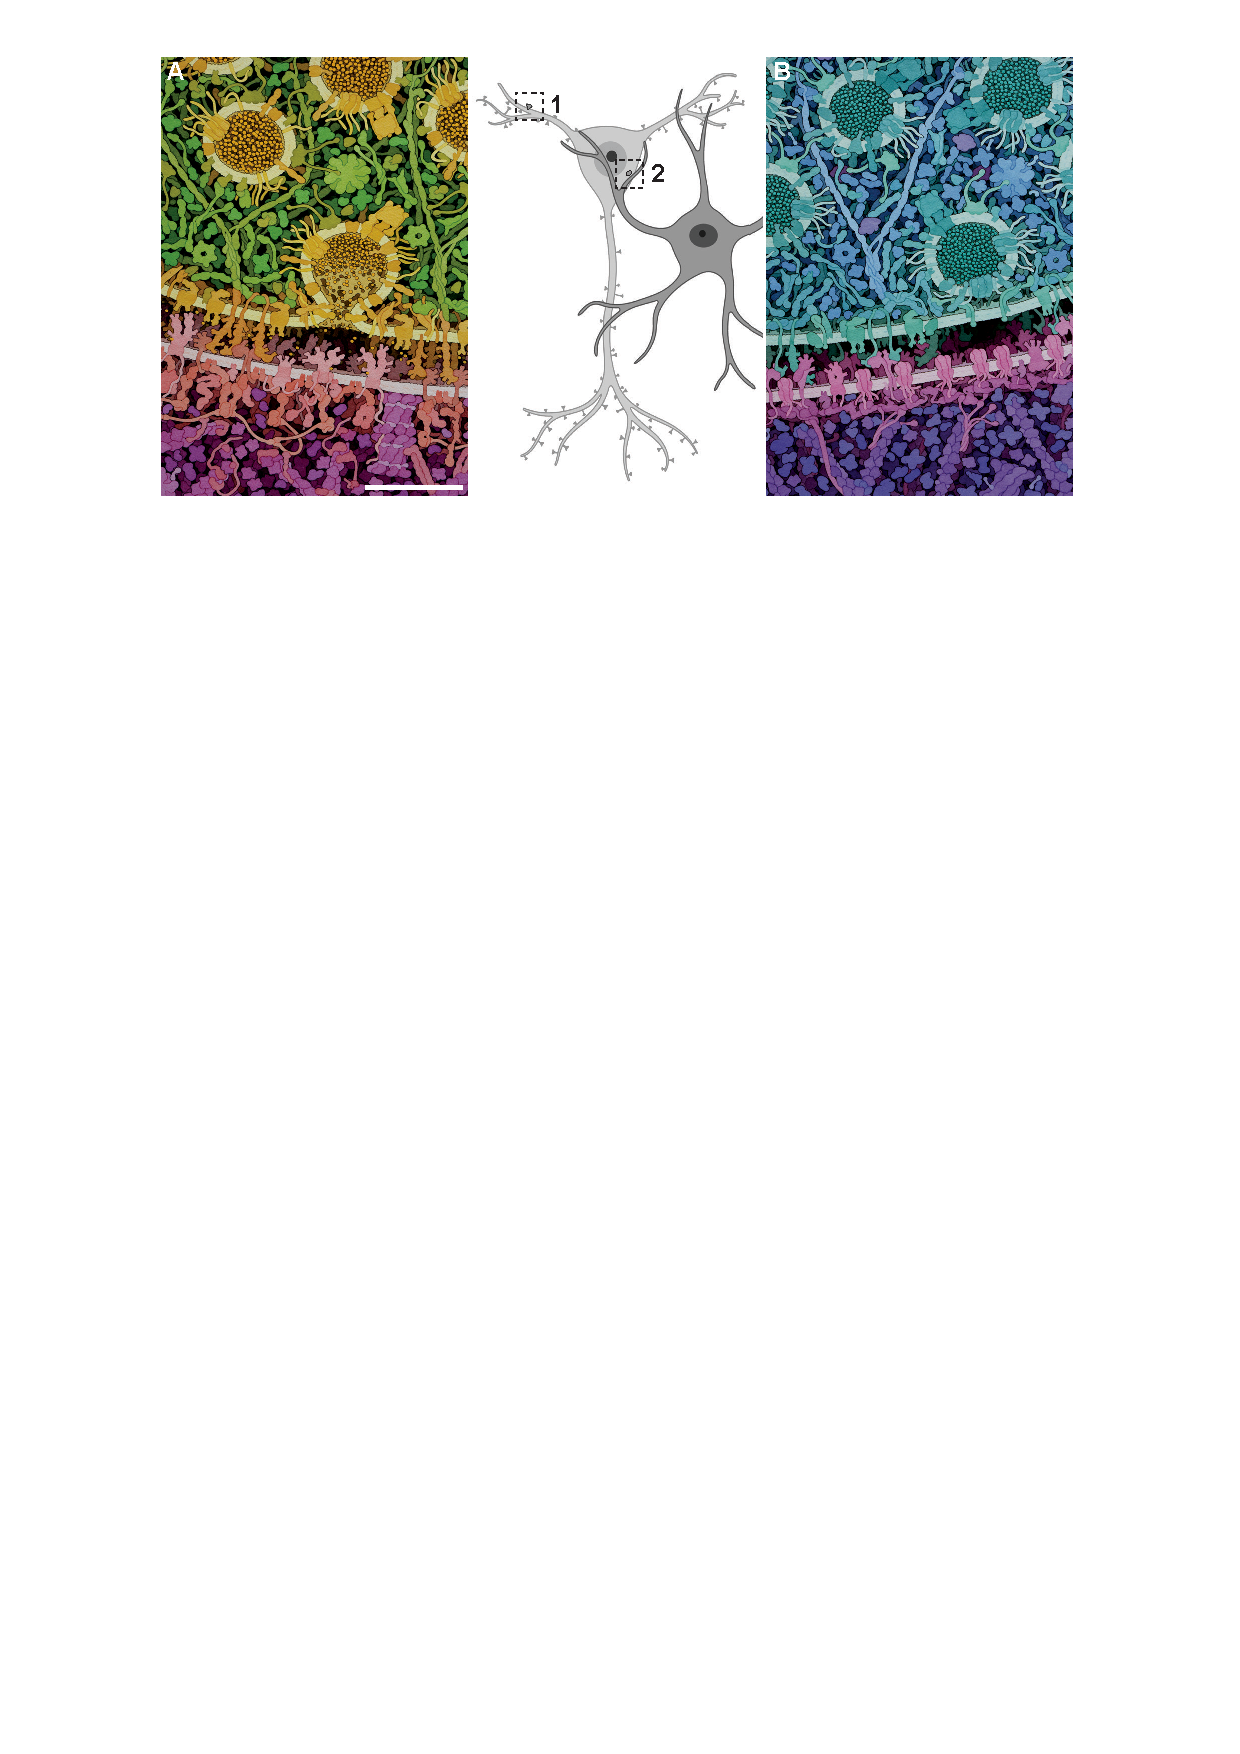
\includegraphics[width=0.7\paperwidth,keepaspectratio]{goodsell}
		\caption[The Central Synapse]{Schematic of an excitatory synapse
			(A) and an inhibitory synapse (B). Excitatory synapses form
			predominately on dendritic spines (inset 1) and are typified by
			their asymmetric shape and a dense postsynaptic accumulation of
			proteins, the excitatory post-synaptic density.  Inhibitory synapses
			form on target a neuron's dendrites, soma (inset 2), and axon.
			Artwork by in (A) and (B) by David Goodsell \cite{Goodsell2020}.
			Scale bar in (A) $\sim$ 40 nm.}
		\label{fig:goodsell}
	\end{center}
\end{figure}


\section{Compact Enumeration}

\lipsum[2-3]
\begin{compactenum} % customize symbol with: \begin{compactitem}[$\circ$]
	\item{First item}
	\item{Second item}
\end{compactenum}


\subsection{Referencing labels}

You can create labels with the \texttt{label} command. Then point to that part
of the document with \texttt{autoref}. For example, "In \autoref{chap:02}, I discuss methods
for testing for differential abundance in protein proteomics experiments."


%% ---- chapter 02

\chapter{My Second Chapter}
\label{chap:02}

\section{Equations}

Statistical testing in proteomics is usually done for each protein-level subset
of the data. The simplest model includes a single fixed-effect term,
Condition which represents experimental treatment groups such as
Genotype (e.g. WT versus Mutant) or Treatment (e.g. BioID versus Control).
Consider the following linear model, given in matrix form, which is fit to the
data from a single protein:
\begin{equation}
	\label{eq:lm}
	Y_{p} = X\beta_{p} + \epsilon_{p} % Y = XB + e
\end{equation}

$Y_{p}$ is a vector of $log_{2}$ intensity for protein $p$. The matrix $X$
stores information about the experiment's fixed-effect covariate,
Condition.  $\beta_{p}$ is a vector of regression coefficients,
obtained from the fit model.  We also estimate $\epsilon_{p}$ which quantifies
any residual error and by definition is normally and independently distributed:
\begin{equation}
    \label{eq:error}
	\epsilon_{p} \stackrel{iid}{\sim} N(0,\sigma^2) % e = N(0,s2)
\end{equation}

Linear, fixed-effect models can be extended to include additional mixed-effects
to provide a description of more complex sources of variation in an experimental
design \cite{Bates2015}:
\begin{equation}
	\begin{gathered}
		\label{eq:lmer}
		Y_{p} =  Z\alpha_{p} + X\beta_{p} + \epsilon_{p} \\
		\alpha_{p} \stackrel{iid}{\sim} N(0,\sigma_{Z}^2) \\
	\end{gathered}
\end{equation}

The mixed-effect term, $Z\alpha_{p}$, includes $Z$, a matrix of mixed-effects.
The parameter $\alpha_{p}$ quantifies error among these mixed-effects (also
called random effects).  By definition, the random-effect error is independently
and normally distributed (Equation \ref{eq:lmer}). Using linear mixed-models we
can untangle variance attributed to a biological effect of interest from other
sources of variation which mask this response.


\section{Example Table}

Put the table (Table \ref{table:example}) caption above its contents.

\begin{table}[ht]
	\caption[This is my table's caption.]{
		Here is a description of my table.}
	\begin{tabular}{lrr}
		\hline
		\textbf{Column 1} & \textbf{Column 2} & \textbf{Column 3} \\
		\hline
		A & 74 & 122\\
		B & 90 & 66\\
		C & 85 & 153\\
		D & 88 & 88\\
		\hline
	\end{tabular}
	\label{table:example}
\end{table}


%% ---- chapter XX

\chapter{Putting Figure Captions on the Second Page}
\label{chap:04}

\begin{figure}[ht] 
	\begin{center}
		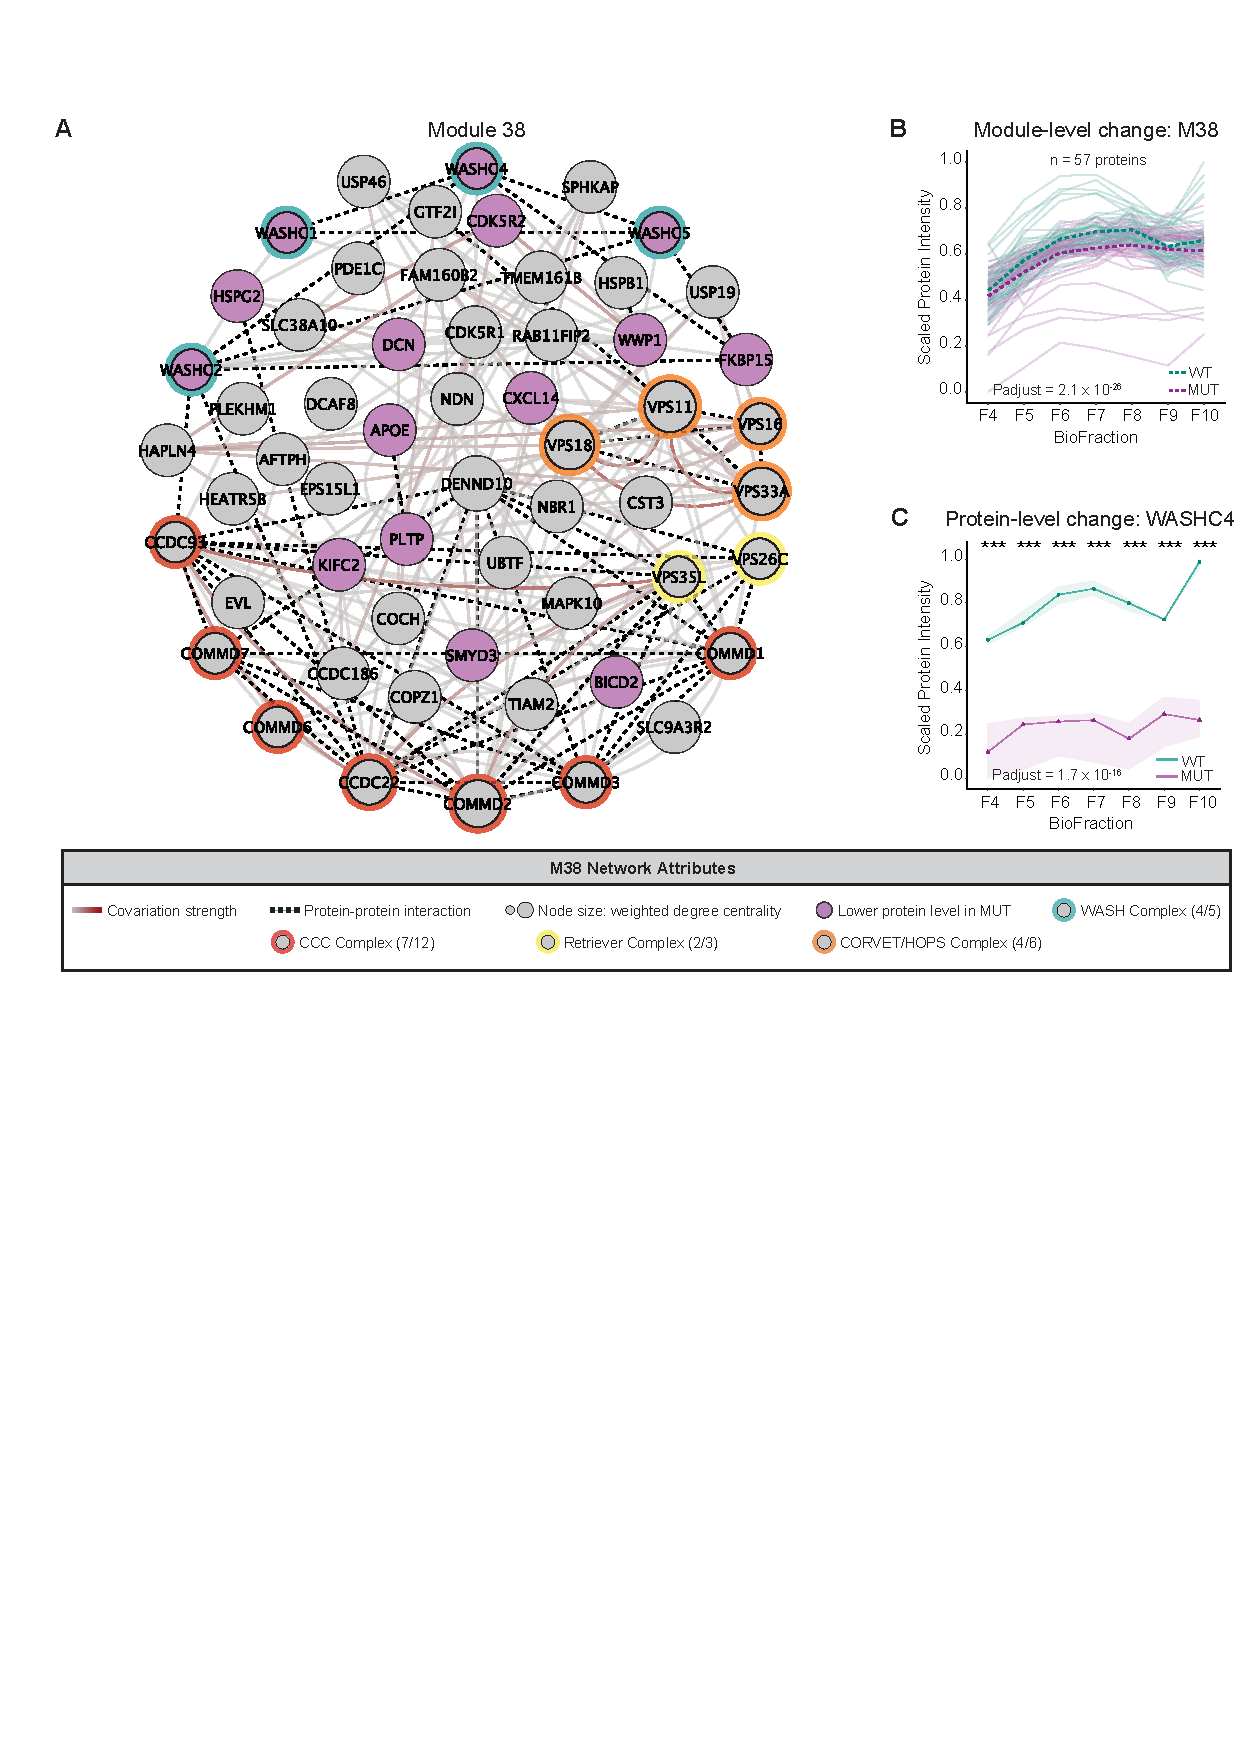
\includegraphics[width=0.7\paperwidth,keepaspectratio]{m38}
			\caption[This is a figure caption.]{Figure adapted from
			\cite{Courtland2021}. Figure caption continued on next page.}
		\label{fig:m38}
	\end{center}
\end{figure}

\begin{figure}[t]
		\contcaption{\lipsum[3]}
\end{figure}


%% ---- chapter XX

\chapter{Conclusions}

% "Conclusion/ s" should be the last chapter in your work
\lipsum[1-3]


%% ---- references

% puts bibliography in Contents
\startbibliography{}

%\nocite{*} % cite all
\begin{singlespace} % force single spaced within entries
\bibliographystyle{unsrtnat}
\bibliography{bibliography}
\end{singlespace}


%% ---- biography

%\chapter{Biography}
%
%%\biography
%
%You cannot include personal details or resume items in your biography... This
%sort of defeats the purpose of any biography. It's not required, and you've
%done so much already, so why bother?


%% ---- end

\end{document}
